\documentclass[11pt,a4paper,twoside,spanish]{book}

\usepackage[utf8]{inputenc}
\usepackage{pkgs/TFG}

\usepackage{amsfonts, amsmath, amssymb, amsthm}
\usepackage{hyperref}
\usepackage{tikz,pgfplots,pkgs/quiver}
\usetikzlibrary{positioning, babel}
\pgfplotsset{compat=1.18}

\usepackage{verbatim}


%\newcommand{\Z}{\mathbb{Z}}
%\newcommand{\N}{\mathbb{N}}




\DeclareMathOperator{\SylowSubgroup}{Syl}
\DeclareMathOperator{\Normalizer}{N}
\DeclareMathOperator{\Center}{Z}
\DeclareMathOperator{\mcd}{mcd}
%\DeclareMathOperator{\Ker}{Ker}
\DeclareMathOperator{\Image}{Im}
%\DeclareMathOperator{\Hom}{Hom}
\DeclareMathOperator{\Aut}{Aut}
\DeclareMathOperator{\Inn}{Inn}
\DeclareMathOperator{\Out}{Out}
\DeclareMathOperator{\Ext}{Ext}
\DeclareMathOperator{\car}{car}


\newcommand{\Syl}[2]{\SylowSubgroup_#1(#2)}
\newcommand{\Norm}[2]{\Normalizer_#1(#2)}
\newcommand{\norm}{\trianglelefteq}
\newcommand{\ord}[1]{\vert#1\vert}
\newcommand{\homo}[3]{#1\colon #2\to #3}
\newcommand{\extension}[5]{1\xrightarrow{} #3 \xrightarrow{#1} #4\xrightarrow{#2} #5 \xrightarrow{} 1}
%\def\mcd{\mathop{\rm mcd}\nolimits}

%\includeonly{Extensiones/split.tex}
\begin{document}
\renewcommand{\tablename}{Tabla}
\frontmatter

\titulo{Cosa nose}
\nombre{Carlos Moya García}
\director{Jon González Sánchez}
\otrodirector{}
\fecha{}

%\maketitle
\thispagestyle{empty}
\pagestyle{plain}
\tableofcontents
\clearpage{\pagestyle{empty}\cleardoublepage}
\pagestyle{fancy}
\fancyhf{}
\renewcommand{\chaptermark}[1]{\markboth{#1}{}}
\fancyhead[LO]{\slshape\nouppercase{\leftmark}}
\fancyhead[RO]{\thepage}
\fancyhead[LE]{\thepage}
\fancyhead[RE]{\slshape\nouppercase{\rightmark}}

%\incluir{Introduccion}

\mainmatter
\renewcommand{\chaptermark}[1]{\markboth{\chaptername\ \thechapter. #1}{}}
% Extensiones
% !TeX root=../tfg2.tex

\chapter{Sucio}

%Esto son cosas a sucio para meter en el capítulo de extensiones o en uno previo de cohomología.

\begin{definicion}
	Un $2$-cociclo $\homo c {Q\times Q} A$ se dice que es normalizado cuando $c(1,1)= 0$
\end{definicion}

% esto tb es cierto para un cociclo no normalizado con accion trivial
\begin{proposicion}
	Sea $\homo c {Q\times Q} A$ un $2$-cociclo normalizado. Entonces para todo $q\in Q$
	\begin{equation*}
		c(1,q)=0=c(q,1)
	\end{equation*}
	\begin{demostracion}
		Evaluando la condición de un $2$-cociclo en $(1,1,q)\in Q^3$
		\begin{equation*}
			1\cdot c(1,q) - c(1,q) + c(1,q) - c(1,1) = c(1,q) =0
		\end{equation*} 
		De igual manera, evaluando en $(q,1,1)\in Q^3$
		\begin{equation*}
			q\cdot c(1,1) - c(q,1) + c(q,1) - c(q,1) = -c(q,1) = 0
		\end{equation*}
		
	\end{demostracion}
\end{proposicion}

\begin{proposicion}\label{prop:normcoc}
	Todo $2$-cociclo $\homo c {Q\times Q} A$ es cohomologo a un $2$-cociclo normalizado. %Esto es, $\frac{Z^{*n}_\varphi(Q,A)}{B^n_\varphi(Q,A)} = \frac{Z^n_\varphi(Q,A)}{B^n_\varphi(Q,A)}$
	\begin{demostracion}
		Sea $c(1,1) = x$. Tomamos una función $\homo \phi Q A$ tal que $\phi(1) = -x$ y construímos el $2$-coborde asociado a $\phi$
		\begin{equation*}
			b(q_1,q_2) = q_1\cdot \phi(q_2) - \phi(q_1q_2) + \phi(q_1)
		\end{equation*}
		$b$ verifica que $b(1,1) = \phi(1) = -x$ y por tanto el cociclo $\tilde c = c+b$ es un cociclo normalizado.
	\end{demostracion}
\end{proposicion}



\begin{ejercicio}
	Estudiar las extensiones salvo equivalencia de $\Z_p$ por $\Z_p$. % y ver que $H^2(\Z_p,\Z_p) \cong \Z_p$.
	
		Los grupos de orden $p^2$ son abelianos y por tanto $\Z_p$ es central en la extensión y la acción es trivial.
		Observamos que si $[c]\in H^2(\Z_p,\Z_p)$ $p[c] = [0]$, por lo que $H^2(\Z_p,\Z_p)$ es un $p$-grupo abeliano de exponente $p$, es decir, isomorfo a $\Z_p^k$ para algún $k\in \N$.
		
		Contando el número de extensiones veremos que $0<k<2$ y por tanto, el número de extensiones equivalentes debe ser $p$.
		
		\textit{(Extensiones isomorfas a $\Z_p\times \Z_p$).}
		\begin{equation*}
			\extension i \pi {\Z_p} {\Z_p\times \Z_p} {\Z_p}
		\end{equation*}
		
		La proyección $\homo \pi {\Z_p\times \Z_p} {\Z_p}$ viene dada por las imágenes de los generadores $e_1=(1,0)$ y $e_2=(0,1)$. Como $\pi$ es sobreyectiva, $\pi(e_1)$ o $\pi(e_2)$ es distinto de la identidad, supongamos que $e_1\notin \Ker(\pi)$. Entonces $\langle e_1 \rangle$ es una escisión de $\pi$ y la extensión es trivial, por lo que se corresponde con el elemento neutro de $H^2$ y es única salvo equivalencia.
		
		\textit{(Extensiones isomorfas a $\Z_{p^2}$).}
		\begin{equation*}
			\extension {i_n} {\pi_n} {\Z_p} {\Z_{p^2}} {\Z_p}
		\end{equation*}
		
		$\Z_{p^2}$ es cíclico y $\Z_p$ debe incluirse en el único subgrupo de $\Z_{p^2}$ de orden $p$. 
		
		Hay $p-1$ formas de incluir $\Z_p$ en $\langle p \rangle \leq \Z_{p^2}$ que se corresponden con los distintos automorfismos de $\langle p \rangle$. Las inclusiones $i_n$ vienen dadas por $i_n(x) = pnx \mod p^2$
		
		Las proyecciones $\pi_n$ vienen dadas por la imagen del $1\in \Z_{p^2}$, que puede mandarse a cualquier elemento no trivial de $\Z_p$ y por tanto hay $p-1$ proyecciones distintas definidas por $\pi_n(1) = n \mod p$ para $n=1\ldots p-1$.
		
		En total, hay $(p-1)^2$ formas de componer las $i_n$ y $\pi_n$. Sumando la extensión trivial dan un total de $p^2-2p+2$, que es menor que $p^2$ y mayor que $1$ para todo primo $p$. 
		
		\textit{(Representantes de las extensiones y cociclos asociados).} 
		La primera extensión es única salvo equivalencia y podemos tomar la inclusión en la primera coordenada $i(x) = (x,0)$ y la proyección en la segunda $\pi(x,y) = y$. El cociclo asociado $c_0$ es trivial ya que la extension escinde.
		
		Para la segunda extensión podemos fijar la inclusión $i_1$ para simplificar cálculos. Sean $n,m\in \{1,\ldots,p-1\}$ distintos y tomemos las proyecciones $\pi_m$ y $\pi_n$. Supongamos que existe un homomorfismo $f$ que haga al siguiente diagrama conmutativo
		\[\begin{tikzcd}
			1 & {\Z_p} & {\Z_{p^2}} & {\Z_p} & 1 \\
			1 & {\Z_p} & {\Z_{p^2}} & {\Z_p} & 1
			\arrow[from=1-1, to=1-2]
			\arrow["{i_1}", from=1-2, to=1-3]
			\arrow["{\pi_m}", from=1-3, to=1-4]
			\arrow[from=1-4, to=1-5]
			\arrow[from=2-1, to=2-2]
			\arrow["{i_1}", from=2-2, to=2-3]
			\arrow["{\pi_n}", from=2-3, to=2-4]
			\arrow[from=2-4, to=2-5]
			\arrow[shift left=1, no head, from=1-2, to=2-2]
			\arrow[shift left=1, no head, from=2-2, to=1-2]
			\arrow["f"', from=1-3, to=2-3]
			\arrow[shift left=1, no head, from=1-4, to=2-4]
			\arrow[shift left=1, no head, from=2-4, to=1-4]
		\end{tikzcd}\]

		Por un lado, $f(i_1(1)) = i_1(1) = p$ y por tanto $f(p)=p$. Por otro lado, $\pi_n(f(1)) = \pi_m(1) = m$ y $f(1)\in \pi_n^{-1}(m) = n^{-1}m + \langle p\rangle$. Esto es absurdo ya que $f(p) = pf(1) = pn^{-1}m \neq p$ pero $n\neq m$. Esto prueba que las extensiones $(\Z_{p^2},i_1,\pi_n)$ son inequivalentes para todo $n=1,\ldots,p-1$.
		
		Una sección de $\pi_n$ es $s_n$ definida por $s_n(x) = n^{-1}x \mod p = \overline{n^{-1}x}$. En efecto, $\pi_n(s_n(x)) = \pi_n(\overline{n^{-1}x}) = nn^{-1}x = x$ para $x=0,\ldots,p-1$.
		El cociclo asociado a esta sección es 
		\begin{equation*}
			c_n(x,y) = i_1^{-1}(s_n(x)+s_n(y)-s_n(x+y)) = \frac{\overline{n^{-1}x}+\overline{n^{-1}y}-\overline{n^{-1}(x+y)}}{p} %= i_1^{-1}\left(\overline{n^{-1}x}+\overline{n^{-1}y}-\overline{n^{-1}(x+y)}\right) 
		\end{equation*}
		
		Como $H^2$ es cíclico, podemos tomar $c_1$, cuya expresión es sencilla, y generar el resto de los cociclos con él
		
		\[
		    c_1(x,y) = \frac{\overline{x} + \overline{y} - \overline{x+y}}{p} =  \begin{cases}
		        0 & \text{si } x+y < p\\
		        1 & \text{si } x+y \geq p
		        \end{cases}
		\]
		% comprobar si se corresponden con los pi_n o estan permutados por un n^-1 o algo asi
		\[
		    c_n(x,y) = nc_1(x,y) =  \begin{cases}
		        0 & \text{si } x+y < p\\
		        n & \text{si } x+y \geq p
		        \end{cases}
		\]

\end{ejercicio}


%\begin{proposicion}
%	\begin{demostracion}
%		A partir de las extensiones $E_1$ y $E_2$ se construye la extensión del producto directo tomando la inclusión y proyección coordenada a coordenada. El objetivo será utilizar los cociclos $c_1$ y $c_2$ para construir una sucesión exacta $1\xrightarrow{} A\xrightarrow{i_3} E_3\xrightarrow{\pi_3} Q \xrightarrow{} 1$ cuyo cociclo asociado sea $c_3=c_1+c_2$.
%		\begin{equation}
%			1\xrightarrow{} A\times A \xrightarrow{i_1\times i_2} E_1\times E_2\xrightarrow{\pi_1\times\pi_2} Q\times Q \xrightarrow{} 1 % comprobar que es exacta
%		\end{equation}
%		La sección $s_1\times s_2$ de $\pi_1\times \pi_2$ tiene como cociclo asociado
%		\begin{align}
%			(c_1\times c_2)\colon (Q\times Q)\times (Q\times Q) &\to A\times A \\
%			                              ((q_{11},q_{12}),(q_{21},q_{22})) &\mapsto (c_1(q_{11},q_{12}),c_2(q_{21},q_{22})) % comprobar el orden de la operacion
%		\end{align}
%		Proyectando $A\times A$ sobre $A$ y haciendo la suma de componentes en $A$ movemos $(c_1\times c_2)((q_{11},q_{12}),(q_{21},q_{22}))$ a $c_1(q_{11},q_{12}) + c_2(q_{21},q_{22})$. Basta identificar $q_{11}$ con $q_{21}$ y $q_{12}$ con $q_{22}$ mediante $\homo \Delta Q {Q\times Q}$ definido por $\Delta(q)=(q,q)$. Notese que el morfismo diagonal está definido para las secciones $s_1$ y $s_2$, por tanto, para los cociclos estará definido de $Q\times Q$ en $(Q\times Q)\times (Q\times Q)$.
%		
%		\begin{equation}
%			Q\times Q \xrightarrow{\Delta} (Q\times Q)\times (Q\times Q) \xrightarrow{c_1\times c_2} A\times A\xrightarrow{+} A
%		\end{equation}
%		El cociclo que buscamos es $c_3=+\circ (c_1\times c_2)\circ \Delta=c_1+c_2$
%		
%		Completando el diagrama de $\Delta$ y $\pi_1 \times \pi_2$ con $\homo i {\tilde E} {E_1\times E_2}$ y $\homo {\tilde\pi} E Q$, para $x\in \tilde E$ $(\pi_1(i(x)),\pi_2(i(x)))=(\tilde\pi(x),\tilde\pi(x))$ lo que implica que $\pi_1(i(x))=\pi_2(i(x))$ y por tanto $i(x)\in E_1\times_Q E_2$. Lo natural es tomar $\tilde E = E_1\times_Q E_2$, $i$ la inclusión y $\tilde\pi(e_1,e_2)=\pi_1(e_1)=\pi_2(e_2)$.
%		
%		% https://q.uiver.app/?q=WzAsNCxbMCwwLCJFXzFcXHRpbWVzIEVfMiJdLFsyLDAsIlFcXHRpbWVzIFEiXSxbMiwxLCJRIl0sWzAsMSwiXFx0aWxkZSBFIl0sWzMsMCwiaSJdLFsxLDAsInNfMVxcdGltZXMgc18yIl0sWzIsMSwiXFxEZWx0YSJdLFsyLDMsIlxcdGlsZGUgcyJdXQ==
%		\[\begin{tikzcd}
%			{E_1\times E_2} && {Q\times Q} \\
%			{\tilde E} && Q
%			\arrow["i", from=2-1, to=1-1]
%			\arrow["{\pi_1\times \pi_2}", from=1-1, to=1-3]
%			\arrow["\Delta", from=2-3, to=1-3]
%			\arrow["{\tilde \pi}", from=2-1, to=2-3]
%		\end{tikzcd}\]
%		
%		$\Ker(\tilde \pi) = \{(e_1,e_2)\in E_1\times_Q E_2 \colon \tilde\pi(e_1,e_2)=0\}=\{(e_1,e_2)\in E_1\times_Q E_2 \colon \pi_1(e_1)=\pi_2(e_2)=0\} = A\times A$
%	
%		Por tanto, la sucesión $1\xrightarrow{} A\times A \xrightarrow{\tilde\imath} E_1\times_Q E_2\xrightarrow{\tilde\pi} Q \xrightarrow{} 1$ es exacta.
%		
%		$i_3(a_1+a_2)=\pi(a_1,a_2)=\pi(a_1+a_2,0)=\pi(0,a_1+a_2)$, para que esté bien definida, tenemos que cocientar $E_1\times_Q E_2$ por $Ker(+)=\{(a_1,a_2)\in A\times A \colon a_1+a_2=0\}=\{(a,-a) \colon a\in A\}$
%		
%		
%		% Fin
%		El cociclo correspondiente a la extensión es por tanto $c_1+c_2$ y por la proposición \ref{extsum} la suma está bien definida en clases de extensiones equivalentes.
%	\end{demostracion}
%\end{proposicion}

% !TeX root=../tfg2.tex

\chapter{Extensiones de grupos}

% introduccion explicar qué se va a hacer, mencionar que se darán interpretaciones de los grupos H^1 y H^2. comentar si eso que el H^3
El objetivo de este capítulo es estudiar todas las formas de construir un grupo $E$ a partir de dos grupos $Q$ y $N$, de tal forma que $E$ tenga un subgrupo normal isomorfo a $N$ y cuyo cociente sea isomorfo $Q$. Para ello, definiremos una relación de equivalencia sobre el conjunto de extensiones y daremos una clasificación usando los grupos de cohomología $H^1$ y $H^2$ (Teoremas \ref{h1} y \ref{h2}).

\section{Equivalencia de extensiones}

% comentar que ya se ha explicado en el cpaitulo anterior las sucesiones exactas etc

\begin{definicion}
	Una extensión de un grupo $Q$ por un grupo $N$ es una sucesión exacta corta
	\begin{equation}\label{eq:ext}
		\extension i \pi N E Q 
	\end{equation}
	Al grupo $N$ lo llamaremos kernel de la extensión, al grupo $Q$ el cociente de la extensión y a $E$ el grupo central de la extensión.
	
	Decimos que otra extensión $\extension {i'} {\pi'} N {E'} Q $ es equivalente si existe un homomorfismo $\homo f E {E'}$ tal que el siguiente diagrama conmuta

	%	\begin{figure}[h!] % quitar figure?
	%		\centering	
			% https://q.uiver.app/?q=WzAsMTAsWzEsMCwiTiJdLFsyLDAsIkUiXSxbMywwLCJRIl0sWzQsMCwiMSJdLFswLDAsIjEiXSxbMCwxLCIxIl0sWzEsMSwiTiJdLFszLDEsIlEiXSxbNCwxLCIxIl0sWzIsMSwiRSciXSxbNCwwXSxbMCwxLCJpIl0sWzEsMiwiXFxwaSJdLFsyLDNdLFs1LDZdLFs2LDksImknIl0sWzksNywiXFxwaSciXSxbNyw4XSxbMiw3LCIiLDEseyJvZmZzZXQiOi0xLCJzdHlsZSI6eyJoZWFkIjp7Im5hbWUiOiJub25lIn19fV0sWzcsMiwiIiwxLHsib2Zmc2V0IjotMSwic3R5bGUiOnsiaGVhZCI6eyJuYW1lIjoibm9uZSJ9fX1dLFsxLDksImYiXSxbMCw2LCIiLDEseyJvZmZzZXQiOi0xLCJzdHlsZSI6eyJoZWFkIjp7Im5hbWUiOiJub25lIn19fV0sWzYsMCwiIiwxLHsib2Zmc2V0IjotMSwic3R5bGUiOnsiaGVhZCI6eyJuYW1lIjoibm9uZSJ9fX1dXQ==
	\begin{equation}\begin{tikzcd}
		1 & N & E & Q & 1 \\
		1 & N & {E'} & Q & 1
		\arrow[from=1-1, to=1-2]
		\arrow["i", from=1-2, to=1-3]
		\arrow["\pi", from=1-3, to=1-4]
		\arrow[from=1-4, to=1-5]
		\arrow[from=2-1, to=2-2]
		\arrow["{i'}", from=2-2, to=2-3]
		\arrow["{\pi'}", from=2-3, to=2-4]
		\arrow[from=2-4, to=2-5]
		\arrow[shift left=1, no head, from=1-4, to=2-4]
		\arrow[shift left=1, no head, from=2-4, to=1-4]
		\arrow["f", from=1-3, to=2-3]
		\arrow[shift left=1, no head, from=1-2, to=2-2]
		\arrow[shift left=1, no head, from=2-2, to=1-2]
	\end{tikzcd}
	\end{equation}
	%\end{figure}
\end{definicion}

El interés está en clasificar todas las extensiones de $Q$ por $N$. La equivalencia de extensiones captura la idea de que los grupos centrales se construyen a partir de $N$ y $Q$ esencialmente de la misma forma, ya que $N$ y $Q$ se incluyen y proyectan de la misma manera. % repetitivo: de la misma forma/manera

A continuación se dan unos ejemplos conocidos de extensiones de grupos.

\begin{ejemplo}
	El grupo diédrico $D_{2n} = \langle a,b\ |\ a^n = b^2 = 1, \ a^b = a^{-1}\rangle$ es una extensión de $C_2=\langle b\rangle$ por $C_n=\langle a\rangle$.
\end{ejemplo}

\begin{ejemplo}
	El grupo alternado $A_n$ se define como el kernel del homomorfimo del signo $\homo {\sgn} {S_n} {\{1,-1\}^\times}$ que manda una permutación a $1$ si es producto de un número par de transposiciones, y a $-1$ si es un número impar. Por tanto, $S_n$ es una extensión de $C_2$ por $A_n$.
	\begin{equation*}
		\extension i {sgn} {A_n} {S_n} {C_2}
	\end{equation*}
\end{ejemplo}

\begin{ejemplo}
	Siguiendo el ejemplo anterior, dado un cuerpo $\mathbb K$ y $n\in \Z^+$, el grupo especial lineal $\SL_n(\mathbb K)$ es el grupo de las matrices $n\times n$ sobre $\mathbb K$ con determinante $1$. $\SL_n(\mathbb K)$ es precisamente el kernel del homomorfismo determinante $\homo \det {\GL_n(\mathbb K)} {\mathbb K^\times}$. Así, $\GL_n(\mathbb K)$ es una extensión de $\mathbb K^\times$ por $\SL_n(\mathbb K)$.
	\begin{equation*}
		\extension i \det {\SL_n(\mathbb K)} {\GL_n(\mathbb K)} {\mathbb K^\times}
	\end{equation*}
\end{ejemplo}

\begin{ejemplo}
	Dados dos grupos $G$ y $H$, se construye la extensión trivial $\extension i \pi  G {G\times H} H$ con $G\times H$ el producto directo e $i$ y $\pi$ la inclusión y proyección canónicas.
\end{ejemplo}

\begin{ejemplo}
	Más generalmente, dados dos grupos $G$ y $N$ y una acción de grupos $\homo \varphi G {Aut(N)}$, el producto semidirecto $N\rtimes_\varphi G$ es una extensión de $G$ por $N$.
\end{ejemplo}

% reeescribir demostracion
\begin{observacion}\label{prop:eqiso}
	Por la Proposición \ref{prop:sflem}, dos extensiones equivalentes $\extension {i_{j}} {\pi_j} N {E_j} Q$ para $j=1,2$ dan lugar a grupos centrales isomorfos.
\end{observacion}

El siguiente ejemplo muestra que el recíproco no es cierto, y por tanto la equivalencia de extensiones es más fuerte que tener grupos centrales isomorfos. 
% ejemplo, poner dem en apendice?
\begin{ejemplo}
	Las extensiones $\extension {\times 3} {\times n} {\Z_3} {\Z_9} {\Z_3}$ para $n=1,2$ no son equivalentes.
	% https://q.uiver.app/?q=WzAsMTAsWzAsMCwiMSJdLFsxLDAsIlxcbWF0aGJie1p9XzMiXSxbMiwwLCJcXG1hdGhiYntafV85Il0sWzMsMCwiXFxtYXRoYmJ7Wn1fMyJdLFs0LDAsIjEiXSxbMCwxLCIxIl0sWzEsMSwiXFxtYXRoYmJ7Wn1fMyJdLFsyLDEsIlxcbWF0aGJie1p9XzkiXSxbMywxLCJcXG1hdGhiYntafV8zIl0sWzQsMSwiMSJdLFswLDFdLFsxLDIsIlxcdGltZXMgMyJdLFsyLDMsIlxcdGltZXMgMSJdLFszLDRdLFs1LDZdLFs2LDcsIlxcdGltZXMgMyJdLFs3LDgsIlxcdGltZXMgMiJdLFs4LDldLFsxLDYsIiIsMSx7Im9mZnNldCI6LTEsInN0eWxlIjp7ImhlYWQiOnsibmFtZSI6Im5vbmUifX19XSxbNiwxLCIiLDEseyJvZmZzZXQiOi0xLCJzdHlsZSI6eyJoZWFkIjp7Im5hbWUiOiJub25lIn19fV0sWzIsNywiZiIsMl0sWzMsOCwiIiwxLHsib2Zmc2V0IjotMSwic3R5bGUiOnsiaGVhZCI6eyJuYW1lIjoibm9uZSJ9fX1dLFs4LDMsIiIsMSx7Im9mZnNldCI6LTEsInN0eWxlIjp7ImhlYWQiOnsibmFtZSI6Im5vbmUifX19XV0=
%\[\begin{tikzcd}
%	1 & {\Z_3} & {\Z_9} & {\Z_3} & 1 \\
%	1 & {\Z_3} & {\Z_9} & {\Z_3} & 1
%	\arrow[from=1-1, to=1-2]
%	\arrow["{\times 3}", from=1-2, to=1-3]
%	\arrow["{\times 1}", from=1-3, to=1-4]
%	\arrow[from=1-4, to=1-5]
%	\arrow[from=2-1, to=2-2]
%	\arrow["{\times 3}", from=2-2, to=2-3]
%	\arrow["{\times 2}", from=2-3, to=2-4]
%	\arrow[from=2-4, to=2-5]
%	%\arrow[shift left=1, no head, from=1-2, to=2-2]
%	%\arrow[shift left=1, no head, from=2-2, to=1-2]
%	%\arrow["f"', from=1-3, to=2-3]
%	%\arrow[shift left=1, no head, from=1-4, to=2-4]
%	%\arrow[shift left=1, no head, from=2-4, to=1-4]
%\end{tikzcd}\]
	\begin{demostracion} %$\Z_9$ tiene un único subgrupo de orden $3$ y por tanto la inclusión es única. Para la proyección, se debe mandar el $\bar1$ de $\Z_9$ al $\bar1$ o $\bar2$ de $\Z_3$, lo que da lugar a las dos extensiones mostradas.
		Lo probamos por reducción al absurdo. Supongamos que existe $\homo f {\Z_9} {\Z_9}$ que haga a las dos extensiones equivalentes. Un automorfismo $f$ de $\Z_9$ viene dado por $f(x) = kx$ con $x\in \Z_9$ y $k\in \Z_9^{\times} = \{1,2,4,5,7,8\}$		 
		
		Para que $\pi_2\circ f = \pi_1$, $(\times2\circ f)(x) = 2kx = x \mod 3$, $k \equiv 2 \mod 3$, por lo que $k = 2,5,8$.
		
		Por otro lado, para que $f\circ i_1 = i_2$, $(f\circ \times3)(x) = 3kx = 3x \mod 9$, por lo que $k = 1,4,7$.
		
		Por tanto, no existe un isomorfismo $f$ que haga al diagrama conmutativo y las extensiones no son equivalentes.
	\end{demostracion}
\end{ejemplo}

\begin{proposicion}
	La equivalencia de extensiones es una relación de equivalencia.
	\begin{demostracion}
		\begin{enumerate}
			\item Reflexiva: $E$ es equivalente a $E$ tomando $f=1_E$.
			\item Simétrica: Si $\homo f {E_1} {E_2}$ es una equivalencia, por la Observación \eqref{prop:eqiso}, $\homo {f^{-1}} {E_2} {E_1}$ es una equivalencia. 
			\item Transitiva: Si $\homo f {E_1} {E_2}$ y $\homo g {E_2} {E_3}$ son equivalencias, $g\circ f\circ i_1 = g\circ i_2 = i_3$ y $\pi_1 \circ g \circ f = \pi_2 \circ f = \pi_3$, entonces $\homo {g\circ f} {E_1} {E_3}$ es una equivalencia.
		\end{enumerate}
	\end{demostracion}
\end{proposicion}

El estudio de las extensiones lo haremos haciendo uso de secciones, que se definen a continuación. La idea será tomar una sección y tratar de construir extensiones equivalentes definiendo una operación de grupo sobre el producto $N\times Q$.

\begin{definicion}
	Sea $\homo \pi A B$ un homomorfismo de grupos, una sección $s$ de $\pi$ es una inversa a la derecha de $\pi$, esto es, $\homo s B A$ tal que $\pi \circ s = 1_B$.
\end{definicion}

\begin{observacion}\label{extact}
	Una extensión $\extension i \pi N E Q$ determina, por conjugación por elementos de $E$, un homomorfismo $\homo \alpha E {\Aut(N)}$ definido por
	\begin{equation*} % tecnicamente es i(n) e i(N) pero bueno es inyectiva noseque da igual imagino no creo q se enfade nadie por hacer un pequeño abuso de notacion
		\alpha(g)(n) = \,^gn = gng^{-1}
	\end{equation*}
	
	Entonces, $\alpha(N) = \Inn(N)$ y $\alpha$ induce un homomorfismo  % explicar que esta bien definida
	\begin{align*}
		\tilde\alpha\colon E/N &\to \Out(N) \\
		gN &\mapsto \overline{\alpha(g)} 
	\end{align*}
	
	El homomorfismo $\tilde\alpha$ se conoce como el kernel abstracto de la extensión. % no se usa
	Fijando una sección $s$ de $\pi$, para todo $q\in Q$, la conjugación por $s(q)$ determina un automorfismo $\varphi(s(q))$ de $N$ definido por $\varphi(s(q))(n) = \alpha(s(q))(n)$. 
	
	Notese que la función $\homo \varphi Q {\Aut(N)}$ no es necesariamente un homomorfismo de grupos, pero sí lo es salvo automorfismos internos. En particular, si la sección $s$ es un homomorfismo o el grupo de automorfismos internos de $N$ es trivial, como se estudia en las secciones \ref{sec:split} y \ref{sec:ab}, entonces $\varphi$ sí es un homomorfismo y podremos hablar de grupos de la acción de la extensión. %%?????????????????
\end{observacion}

\begin{observacion}
	Dos extensiones $E$ y $E'$ equivalentes dan lugar a un mismo kernel abstracto.
	\begin{demostracion}
	 	$f\left(i(n)^{s(q)}\right) = i'(n)^{s'(q)}$
	 \end{demostracion}
\end{observacion}

Por ello, para estudiar las extensiones salvo equivalencia procederemos de la siguiente forma.
\begin{enumerate}
	\item Determinar todas las acciones externas de $Q$ en $N$ que dan lugar a una extensión de grupos de $Q$ por $N$.
	\item Para cada acción, construir todas las extensiones de $Q$ por $N$ que dan lugar a esa acción.
	\item Ver cuáles de ellas son equivalentes.
\end{enumerate}
% podemos fijar una acción $\homo \varphi Q {\Aut(N)}$ y estudiar las extensiones que dan lugar a esa acción.

\begin{definicion}
	Sean $Q$ y $N$ grupos y $\varphi$ una acción de $Q$ en $N$. Denotamos por $\Ext_\varphi(Q,N)$ al conjunto de clases de extensiones equivalentes de $Q$ por $N$ que dan lugar a la acción $\varphi$.
\end{definicion}



% !TeX root=../tfg2.tex

\section{Extensiones separables}\label{sec:split}


\begin{definicion}	
	Decimos que una extensión $\extension i \pi N E Q$ es separable cuando existe una sección $\homo s Q E$ de $\pi$ que es un homomorfismo.
\end{definicion}

%G tiene un subgrupo isomorfo a Q, interseca trivialmente con N por ser una sucesion exacta y por tanto es un producto semidirecto...
\begin{teorema}\label{splitext}
	Una extensión $\extension i \pi N E Q$ separable es equivalente a $\extension {} {} N {Q\ltimes_{\varphi} N} Q$, donde $\homo \varphi Q \Aut(N)$ es una acción de grupos de $Q$ en $N$. % explicar que es una accion y no una funcion
	\begin{demostracion}
		Si $E$ es separable, existe una sección $\homo s Q E$ que es homomorfismo. $s$ es inyectiva porque es una inversa por la derecha de $\pi$ y, por tanto, $Q\cong s(Q) \leq E$.
		$\pi (i(N)) = \{1\}$ y $s(q)\in i(N)$ sí y solo sí $q = 1$, por lo que $s(Q)\cap i(N) = {1_E}$ y $E$ es isomorfo a un producto semidirecto externo de $Q$ por $N$.
		
		El isomorfismo $\homo f {Q\ltimes N} E$ viene dado por $(q,n)\in Q\ltimes N$, $f(q,n) = s(q)i(n)$. Para ver que es un isomorfismo basta comprobar que la operación de grupo en $E$ es compatible con la del producto semidirecto.
		
		Sean $n_1,n_2\in N$ y $q_1,q_2\in Q$
		\begin{equation*}
			s(q_1)i(n_1)s(q_2)i(n_2) = s(q_1)s(q_2)i(n_1)^{q_2}i(n_2) = s(q_1q_2)i(n_1^{q_2}n_2) 
		\end{equation*}
		
		Para ver que las extensiones son equivalentes, se toman la inclusión $i'$ y proyección $\pi'$ canónicas de $Q\ltimes N$ y se verifica trivialmente que $i=f \circ i'$ y $\pi = \pi' \circ f$.
		% <=
		%En la otra dirección, definiendo para $n\in N, \ q\in Q$ $i(n) = (1_Q,n)$ y $\pi((n,q)) = qN$ % TODO
	\end{demostracion}
\end{teorema}


% Splittings (Escisiones)
\subsection{Clasificación de las escisiones}

Hemos visto que las extensiones separables son únicas salvo equivalencia. A continuación, tomaremos la extensión separable canónica

\begin{equation}\label{extsplit}
	\extension i \pi A {Q \ltimes A} Q
\end{equation}
y daremos una clasificación de todas las escisiones posibles de la extensión cuando A es abeliano.
% caso no abeliano H^1 blablabla

\begin{definicion}
	Diremos que dos escisiones $s_1$ y $s_2$ son $A$-conjugadas si existe un $a\in A$ tal que $s_1(q)=s_2(q)^{i(a)}$ para todo $q\in Q$
\end{definicion}

% escisiones vienen dadas por 1-cociclos
\begin{proposicion}
	Las escisiones de \eqref{extsplit} son homomorfismos de la forma $s(q) = (q,c(q))$ donde $\homo c Q A$ es un $1$-cociclo.
	\begin{proof}
		Una sección $s$ de $\pi$ tiene la forma $s(q) = (q,c(q))$ donde $c$ es una función $\homo c Q A$. Imponiendo que la sección sea un homomorfismo
		\begin{align*}
			s(q_1)s(q_2) &= (q_1q_2,c(q_1)\cdot q_2 + c(q_2)) \\
			s(q_1q_2) &= (q_1q_2,c(q_1q_2))
		\end{align*}
		la función $c$ tiene que verificar la ecuación de un $1$-cociclo para que $s$ sea una escisión.
		\begin{equation}
			c(q_1q_2) = c(q_1)\cdot q_2 + c(q_2)
		\end{equation}
	\end{proof}
\end{proposicion}



\begin{proposicion}
	Sean $s_1$ y $s_2$ dos escisiones y $c_1$ y $c_2$ los $1$-cociclos asociados. Entonces $s_1$ y $s_2$ son $A$-conjugadas si $c_1$ y $c_2$ se diferencian en un $1$-coborde.
	\begin{demostracion}
		Si existe un $a \in A$ tal que $s_1(q) = s_2(q)^{i(a)}$ para todo $q\in Q$, 
		\begin{align*}
		(q,c_1(q)) &= (1,-a)(q,c_2(q))(1,a) \\
					&= (q,-a \cdot q +  c_2(q) + a)
		\end{align*}
		
		La diferencia entre $c_1$ y $c_2$ verifica la ecuación de un $1$-coborde
		
		\begin{equation}
			c_2(q) - c_1(q) = a\cdot q - a
		\end{equation}
	\end{demostracion}
\end{proposicion}

%\begin{observacion}
%	Las definiciones de $1$-cociclos y $1$-cobordes dadas se corresponden con las definiciones usuales en el caso en que $N$ es abeliano.
%	\begin{align}
%		c(q_1q_2) = c(q_1)^{q_2}c(q_2) = c(q_1)\cdot q_2 + c(q_2) \\
%		c_1(q) = n^{-q}c_2(q)n \iff c_2(q)-c_1(q) = n\cdot q - n
%	\end{align}
%\end{observacion}

% explicar que se corresponde con el grupo de cohomologia en el caso abeliano
\begin{teorema}\label{h1}
	Sea $E$ una extensión separable de $Q$ por $A$. Entonces, las clases de escisiones $A$-conjugadas están en correspondencia uno a uno con los elementos de $H^1(Q,A)$.
\end{teorema}

% se comprueba trivialmente que es una relacion de equivalencia
% !TeX root=../tfg2.tex

\section{Extensiones con kernel abeliano}\label{sec:ab}

A continuación estudiaremos el caso en que $N$ es un grupo abeliano que a partir de ahora denotaremos por $A$. 

Por la Observación \ref{extact}, como $\Inn(A)$ es trivial, $Out(N)=Aut(N)$ y la acción de $Q$ en $A$ es un homomorfismo de grupos, lo que hace a $A$ un $Q$-módulo. A partir de ahora, fijaremos una acción de $Q$ en $A$ y estudiaremos todas las extensiones que dan lugar a dicha acción.

\begin{equation}\label{exta}
	1\to A\xrightarrow{i} E\xrightarrow{\pi} Q\to 1
\end{equation}

\begin{equation}
	\varphi \colon Q \to Aut(A)
\end{equation}

% suena raro lo del axioma de eleccion aprende a escribir
Para estudiar esta extensión, consideramos una sección $s$ de $\pi$, que en el caso de $Q$ infinito se puede asegurar que existe asumiendo el axioma de elección. Como $Q\cong E/i(A)$, dados $g,h\in Q$, $\pi\left(s(g)s(h)s(gh)^{-1}\right) = 1_{Q}$ por ser $\pi$ homomorfismo. Por tanto, $s(gh)$ y $s(g)s(h)$ distan en un elemento de $i(A)$ y podemos definir una función $\homo c {Q\times Q} {A}$ que mide cuánto dista $s$ de ser un homomorfismo

\begin{equation}\label{eq:factorsystem}
	s(g)s(h) = i\left(c(g,h)\right)s(gh)
\end{equation}

Podemos recuperar la extensión \eqref{exta} a partir de la acción $\varphi$ que hemos fijado y de la función $c$. 
Como $E=\bigcup\limits_{q\in Q} i(A)s(q) = i(A)s(Q)$ es una unión disjunta, podemos expresar unívocamente cada elemento de $E$ como un producto de elementos de $i(A)$ y $s(Q)$. Es decir, tenemos una biyección $A\times Q \to E$. A partir del producto en $E$, podemos definir una operación de grupo en $A\times Q$, que denotaremos por $E_{c}$. Dados $(a_1,q_1),(a_2,q_2)\in A\times Q$ tenemos:
\begin{align}\begin{split}
i(a_1)s(q_1)i(a_2)s(q_2) &= i(a_1)i(q_1\cdot a_2)s(q_1)s(q_2) \\ &= i(a_1+ q_1\cdot a_2 + c(q_1,q_2))s(q_1q_2)
\end{split}\end{align}
\noindent Por tanto, la operación en $E_c$ viene dada por:

\begin{equation}\label{extop}
(a_1,q_1)(a_2,q_2) = (a_1 + q_1\cdot a_2 + c(q_1,q_2),q_1q_2)
\end{equation}

Notese que este producto no depende directamente de la sección $s$ escogida. Por ello, supondremos que la sección $s$ es normalizada 

\begin{equation}
	s(1) = 1
\end{equation}
de donde obtenemos que $c$ verifica la siguiente condición de normalización
\begin{equation}\label{cocnorm}
	c(1,q) = 0 = c(q,1)
\end{equation}
De esta forma, el isomorfismo $\homo f {E_c} E$ viene dado por $f(a,q) = i(a)s(q)$. La inclusión de $A$ a $E_c$ y la proyección a $Q$ son las canónicas, haciendo a la extensión $E_c$ equivalente a \eqref{exta}.

%Queda demostrada la siguiente proposición.
%\begin{proposicion}\label{prop:equivcoc}
%	La extensión $\extension {i'} {\pi'} A {E_c} Q$ es equivalente a \eqref{exta}.
%\end{proposicion}

%La siguiente proposición prueba que una función $\homo c {Q\times Q} A$ define una operación de grupo en $E_c$ con la acción $\varphi$ cuando $c$ es un 2-cociclo.

\begin{proposicion}\label{prop:res1}
Sea $\varphi$ una acción de $Q$ en $A$ y $\homo c {Q\times Q} A$ una función que verifica la condición de normalización \eqref{cocnorm}. Entonces, la operación \eqref{extop} define una extensión de $Q$ por $A$ cuando $c$ es un $2$-cociclo normalizado.
	\begin{demostracion}
	Para ver que la funcion define una operación de grupo comprobamos la asociatividad y la existencia de identidad e inversos.
	%	(a_1+q_1\cdot a_2 + c(q_1,q_2),q_1q_2)(a_3,q_3) = 
%	(a_1+q_1\cdot a_2 + c(q_1,q_2) + q_1q_2\cdot a_3 + c(q_1q_2,q_3),q_1q_2q_3)
	
%	(a_1,q_1)(a_2+q_2\cdot a_3 + c(q_2,q_3),q_2q_3) = 
%	(a_1 + q_1\cdot a_2 + q_1q_2\cdot a_3 + q_1\cdot c(q_2,q_3) + c(q_1,q_2q_3),q_1q_2q_3)
	
%	c(q_1,q_2) + c(q_1q_2,q_3) = q_1\cdot c(q_2,q_3) + c(q_1,q_2q_3)

	\textit{(i) Asociatividad.}
	Imponiendo que para todo $(a_i,q_i)\in A\times Q$ con $i=1,2,3$
	\begin{equation*}
		[(a_1,q_1)(a_2,q_2)](a_3,q_3) = (a_1,q_1)[(a_2,q_2)(a_3,q_3)]
	\end{equation*} 
	llegamos a que $c$ verifica la ecuación de un $2$-cociclo normalizado	
	\begin{equation}\label{eq2coc}	
		 q_1\cdot c(q_2,q_3) - c(q_1q_2,q_3) + c(q_1,q_2q_3) - c(q_1,q_2) = 0
	\end{equation}
	
	\textit{(ii) Identidad.} Comprobamos que $(0,1)$ es la identidad de $E_c$. 
	Sea $(a,q)\in A\times Q$,
	\begin{align*}
		(0,1)(a,q) &= (0 + 1\cdot a + c(1,q), q) = (a,q) \\
		(a,q)(0,1) &= (a+q\cdot 0 + c(q,1),q) = (a,q)
	\end{align*}
	
	\textit{(iii) Inverso.} Se comprueba utilizando \eqref{eq2coc} que el inverso de $(a,q)\in A\times Q$ es $(-q^{-1}\cdot a -c(q^{-1},q),q^{-1})$.
%	\begin{align*}
%		(a,q)(-q^{-1}\cdot a -c(q^{-1},q),q^{-1}) 
%		&= (a+q\cdot (-q^{-1}\cdot a -c(q^{-1},q)) + c(q,q^{-1}),1)   \\
%		&= (a - a - q\cdot c(q^{-1},q)+c(q,q^{-1}),1) \\
%		&= (c(q,1)-c(1,q),1) = (0,1) \\
%		(-q^{-1}\cdot a -c(q^{-1},q),q^{-1})(a,q)
%	\end{align*}
	
	Finalmente, comprobamos que la inclusión $i$ y proyección $\pi$ canónicas de $A\times Q$ son homomorfismos y hacen a la sucesión exacta.
	\begin{equation*}
		i(a_1)i(a_2)=(a_1 + 1 \cdot a_2+c(1,1),1) = (a_1+a_2,1)=i(a_1+a_2)
	\end{equation*}
	\begin{equation*}
		\pi((a_1,q_1)(a_2,q_2))=\pi(-,q_1q_2) = q_1q_2 = \pi(a_1,q_1)\pi(a_2,q_2)
	\end{equation*}
	\begin{equation*}
		\pi(i(a)) = \pi(a,1) = 1
	\end{equation*}
	\end{demostracion}
\end{proposicion}

\begin{proposicion}\label{prop:res2}
	Sea $E$ una extensión de $Q$ por $A$, $s_1$ y $s_2$ dos secciones normalizadas de $Q$ a $E$ y $c_1,c_2$ los cociclos asociados a $s_1$ y $s_2$. Entonces, $c_1$ y $c_2$ se diferencian en un $2$-coborde normalizado y la extensión $E$ determina la clase $[c_1]\in H_\varphi^2(Q,A)$. 
	
	\begin{demostracion}
		La diferencia de $s_1$ y $s_2$ define una función $\homo e Q {A}$ por $s_2(q) = i(e(q))s_1(q)$. Cambiando la sección $s_2$ por $s_1$ en \eqref{eq:factorsystem}
		\begin{align*}
			i(c_2(g,h))s_2(gh) 
			&= s_2(g)s_2(h) \\ 
			&= i(e(g))s_1(g)i(e(h))s_1(h)\\ 
			&= i(e(g) + g \cdot e(h)) s_1(g)s_1(h) \\ 
			&= i(e(g) + g \cdot e(h) + c_1(g,h))s_1(gh) \\
			&= i(e(g) + g \cdot e(h) - e(gh) + c_1(g,h))s_2(gh)
		\end{align*}
		obtenemos que la diferencia de $c_2$ y $c_1$ es el coborde de $e$
		\begin{equation} 
			(c_2-c_1)(g,h) = g \cdot e(h) - e(gh) + e(g)
		\end{equation}
		
		Además, por ser $c_1$ y $c_2$ cociclos normalizados
		\begin{equation*}
			(c_2-c_1)(1,1) = e(1) = 0
		\end{equation*}
		$c_2-c_1$ es un coborde normalizado.
	\end{demostracion}
\end{proposicion}

%En \ref{prop:equivcoc} hemos probado que la extens
Hemos visto en \ref{prop:res1} que un $2$-cociclo normalizado da lugar a una extensión de $Q$ por $A$ y en \ref{prop:res2} que dos extensiones son equivalentes cuando los $2$-cociclos normalizados son cohomólogos. La elección de cociclos normalizados es valida ya que como se ha visto en la Proposición \ref{prop:normcoc}, todo $2$-cociclo es cohomólogo a uno normalizado. En el Apéndice $\ref{apen:norm}$ se da la operación de grupo de $E_c$ para un cociclo no normalizado.

Queda demostrado el siguiente teorema. % Como se dice cuando algo no pierde generalidad

\begin{teorema}\label{h2}
	Sea $A$ un $Q$-módulo dado por una acción $\homo \varphi Q {Aut(A)}$. Entonces, las extensiones salvo equivalencia de $Q$ por $A$ están en correspondencia uno a uno con los elementos del segundo grupo de cohomología.
	\begin{equation*}
		\Ext_{\varphi}(Q,A)\cong H^2_{\varphi}(Q,A)
	\end{equation*}
\end{teorema}

\begin{observacion}\label{obs:split}
	El producto semidirecto se corresponde con el elemento neutro de $H^2(Q,A)$.
	\begin{demostracion}
		Por el Teorema \ref{splitext}, si una sección es un homomorfismo, el $2$-cociclo asociado a ésta es trivial.
	\end{demostracion}
\end{observacion}

% hablar de la estructura de grupo de H2 (suma de cociclos es cociclo): de esto hablo en la definicion de cociclo
% mencionar que es no vacio
\begin{proposicion}\label{extsum}
	Sean $[E_1],[E_2]\in Ext(Q,A)$ dos extensiones y $[c_1],[c_2]\in H^2(Q,A)$ sus cociclos asociados, podemos definir la suma $[E_1] + [E_2]$ como la clase de extensiones equivalentes asociada a $[c1+c2]\in H^2(Q,A)$. Es decir, $Ext_\varphi(Q,A)$ tiene una estructura de grupo abeliano heredada de $H^2(Q,A)$.
\end{proposicion}

En el Apéndice \ref{baersum} se da otra forma de construir la suma anterior sin el uso de cociclos.

\section{Teorema de Schur-Zassenhaus. Caso abeliano}



\begin{teorema}\label{thmschurab} Sea $G$ un grupo finito y sea $N \norm G$ abeliano, $\ord{N}=n$ y $\ord{G:N}=m$ con $\mcd(n,m)=1$. Entonces $G$ contiene subgrupos de orden $m$ y dos cualesquiera son conjugados.
	\begin{demostracion}
%		Tomamos una sección $s$ y su $2$-cociclo asociado $c$. 
%		\begin{equation}
%			c(q_1,q_2)\cdot q_3  - c(q_1,q_2q_3)+ c(q_1q_2,q_3) -c(q_2,q_3) =0
%		\end{equation}
%		Definimos la función ${\displaystyle \tilde c(x) = \sum_{t\in Q} c(t,x)}$ y hacemos la suma en $q_1\in Q$
%		\begin{equation}\label{coccob}
%			m c(q_2,q_3) = \tilde c(q_2)\cdot q_3 + \tilde c(q_3) - \tilde c(q_2q_3)
%		\end{equation}
%		
%		Como $\mcd(m,n)=1$, existe un $k\in \Z$ tal que $km\equiv 1 \mod n$. Multiplicando por $k$ llegamos a 
%		\begin{equation}
%			c(q_2,q_3) = k \tilde c(q_2)\cdot q_3 + k \tilde c(q_3) - k \tilde c(q_2q_3)
%		\end{equation}
%		Por tanto, $c$ verifica la ecuación de un coborde para la función $k \tilde c$ y $H^{2}(Q,N)$ es trivial. Por la Observación \ref{obs:split}, $G$ es un producto semidirecto de $Q$ por $N$.
%		
%		Para ver que dos subgrupos cualesquiera son conjugados, cogemos $s$ una escisión de $G$ y $a$ su $1$-cociclo asociado. 
%		\begin{equation}
%			a(q_1q_2)=a(q_1)\cdot q_2 + a(q_2)
%		\end{equation}
%		Haciendo la suma en $q_1\in Q$ y multiplicando por $k$
%		\begin{equation}
%			a(q_2) = k\tilde a - k\tilde a \cdot q_2
%		\end{equation}
%		vemos que $a$ verifica la ecuación de un $1$-coborde para la función $k\tilde a$ y $H^1(Q,N)$ es trivial. Por el Teorema $\ref{h1}$, todas las escisiones son $N$-conjugadas y por tanto son conjugadas.

		Por el Teorema \ref{thm:trivialH}, $H^2(Q,N)$ es trivial y por la Observación \ref{obs:split}, $G$ es un producto semidirecto de $Q$ por $N$. Esto prueba la parte de existencia.
		
		Para la conjugación, cualquier subgrupo $\tilde Q$ de $G$ de orden $m$, al ser $\mcd(n,m)=1$, tiene intersección trivial con $N$ y la proyección sobre $G/N$ es inyectiva. Por tanto, $\tilde Q$ es una escisión de $G$. Por el mismo teorema, $H^1(Q,N)$ es trivial y por el Teorema \ref{h1} todas las escisiones de la extensión $G$ son $N$-conjugadas y por tanto conjugadas. 
	\end{demostracion}
\end{teorema}
\subsection{Extensiones abelianas}

Un caso particular de \eqref{exta} es cuando la acción de $Q$ en $A$ es trivial

%\incluir{extensions}

%% !TeX root=../tfg2.tex

\chapter{Teoremas de Hall}

%\begin{definicion} 
%	\pi subgrupos
%	O_\pi subgrupos
%\end{definicion}

% explicar que los pi subgrupos generalizan los p-subgrupos, hall subgrupos si existen son conjugados.
\begin{definicion}
	Sea $G$ un grupo y $\pi$ un conjunto no vacío de primos. Llamamos $\pi$-subgrupo de $G$ a un subgrupo cuyo orden es un $\pi$-número, esto es, un número que es producto de primos de $\pi$.
	Definimos un $\pi$-subgrupo de Sylow como un $\pi$-subgrupo maximal y al conjunto de los $\pi$-subgrupos de Sylow lo denotaremos por $\Syl \pi G$.
\end{definicion}
\begin{definicion}
	Un $\pi$-subgrupo $H$ de $G$ decimos que es un $\pi$-subgrupo de Hall si $\ord{G:H}$ es un $\pi'$-número, es decir, un número que no es divisible por ningún primo de $\pi$. Denotaremos por $\Hall \pi G$ al conjunto de los $\pi$-subgrupos de Hall.
\end{definicion}

\begin{observacion}
	Claramente los $\pi$-subgrupos de Hall son $\pi$-subgrupos de Sylow, pero mientras que estos últimos siempre existen, la existencia de los subgrupos de Hall no está garantizada. Por ejemplo, en $A_5$ no hay $\pi$-subgrupos de Hall para $\pi = \{2,5\}, \{3,5\}$ ya que un grupo simple no abeliano no puede tener subgrupos propios de índice menor que 5.% explicar en una proposicion? 
\end{observacion}

\begin{definicion}
	Al subgrupo generado por todos los $\pi$-subgrupos normales de $G$ lo denotamos por $\Core \pi G$. Este subgrupo es a su vez un $\pi$-subgrupo ya que si $H,K\norm G$, $\ord{HK} = \frac{\ord{H}\ord{K}}{\ord{H\cap K}}$ es un $\pi$-número. Además es el único $\pi$-subgrupo normal maximal de $G$.
\end{definicion}

\begin{proposicion}\label{prop:coreint}% al igual q pasa con los p-Sylow
	Sea $G$ un grupo y $\pi$ un conjunto de primos. Entonces, $\Core \pi G$ es la intersección de todos los $\pi$-subgrupos de Sylow de $G$.
	\begin{demostracion}
		Sea $M=\Core \pi G$ y $S\in \Syl \pi G$, entonces $MS$ es un $\pi$-subgrupo. Por maximalidad de $S$, se sigue que $M\leq MS = S$. Por otro lado, la intersección de todos los $\pi$-subgrupos de Sylow es un subgrupo característico y por tanto está contenida en $M$.
	\end{demostracion}
\end{proposicion}

% subgrupos de hall de subgrupo normal y cociente
\begin{proposicion}\label{prop:normalhall}
	Sea $G$ un grupo finito, $N\norm G$ y $H\in \Hall \pi G$. Entonces $H\cap N \in \Hall \pi N$ y $HN/N \in \Hall \pi {G/N}$.
	\begin{demostracion}
		Basta comprobar que $\ord{H\cap N}$ y $\ord{HN/N}$ son $\pi$-números y que $\ord{N:H\cap N}$ y $\ord{G/N:HN/N}$ son $\pi'$-números.
		
		$H\cap N$ es un subgrupo de $H$ y por tanto $\ord{H\cap N}$ es un $\pi$-número. Por ser $N$ normal, $HN$ es un subgrupo y $\ord{N:H\cap N} = \ord{HN:H}$ divide a $\ord{G:H}$ que es un $\pi'$-número. Por tanto, $H\cap N \in \Hall \pi N$.
		
		$\ord{HN:N} = \ord{H:H\cap N}$ es un $\pi$-número y $\ord{\frac{G}{N}:\frac{HN}{N}} = \frac{\ord{G}}{\ord{HN}}$ divide a $\frac{\ord{G}}{\ord{N}}$ por lo que es un $\pi'$-número y $HN/N \in \Hall \pi {G/N}$.
	\end{demostracion}
\end{proposicion}

\begin{teorema}[Schur-Zassenhaus]\label{thm:schur} Sea $G$ un grupo finito y $N\norm G$ un subgrupo de Hall, es decir, $\ord{N}=n$ y $\ord{G:N}=m$ con $\mcd(n,m)=1$. Entonces $G$ contiene subgrupos de orden $m$ y son conjugados. % explicar que G es producto semidirecto de N por Q
	\begin{demostracion}
		El caso $N$ abeliano ya ha sido demostrado en el Teorema \ref{thmschurab}. Basta demostrar la existencia y la conjugación en el caso general.
		
		\textit{(i) Existencia.} Lo demostramos por inducción fuerte sobre el orden de $G$. 
		Podemos tomar como caso base $C_p$, que como es abeliano se cumple el resultado. 
		Para el caso general, tomemos un primo $p$ que divida a $n$ y $P\in \Syl p N$. Sean $L=\Norm G P$ y $C=\Center(P)$.
		Como $C$ es característico en $P$ y $P\norm L$, tenemos que $C\norm L$.
		Por el argumento de Frattini, $G=LN$.
		Observamos que $\ord{L:N\cap L} = \ord{LN:N} = m$ y que $N\cap L \norm L$ por el Segundo Teorema de Isomorfía.
		
		El subgrupo $C$ es no trivial ya que es el centro de un $p$-subgrupo. Aplicando inducción sobre el grupo $L/C$, existe $H/C\leq L/C$ de orden $m$ y volviendo a $G$ por el Teorema de Correspondencia, existe un subgrupo $H$ de índice $m$ en $C$. Aplicando el caso abeliano a $C$ y $H$ se concluye que existe un subgrupo $Q\leq H$ de orden $m$.
%		\begin{figure}[h!]
%			\begin{tikzpicture}[node distance=2cm, scale=1, transform shape]
%				\title{Diagrama}
%				
%				\node(G) {$G$};
%				\node(N)		[below right = 1cm and 3cm of G] {$N$};
%				\node(L)		[below = 1.5cm of G] {$L=N_{G}(P)$};
%				\node(NcL)	[below = 1.5cm of N] {$N\cap L$};
%				\node(P)		[below = 0.5cm of NcL] {$P$};
%				\node(C)		[below = 1.5cm of NcL] {$C=Z(P)$};
%				\node(H)		[below = 1.5cm of L] {$H$};
%				\node(Q)		[below = 1.5cm of H] {$Q$};
%				\node(C1)	[below = 1.5cm of C] {$1$};
%				
%				
%				\draw(G)-- node[above]{$\norm$} node[below]{$m$}(N);
%				\draw(G)--(L);
%				\draw(N)--(NcL);
%				\draw(L)-- node[above]{$\norm$} node[below]{$m$}(NcL);
%				\draw(L)--(H);
%				%\draw(NcL)--(C);
%				\draw(NcL)--(P);
%				\draw(P)--(C);
%				\draw(H)-- node[above]{$\norm$} node[below]{$m$}(C);
%				\draw(H)--(Q);
%				\draw(Q)-- node[above]{$\norm$} node[below]{$m$}(C1);
%				\draw(C)--(C1);
%	
%			\end{tikzpicture}
%		\end{figure}
		
		\textit{(ii) Conjugación (Caso N resoluble)}. Sean $Q_1$ y $Q_2$ subgrupos de $G$ de orden $m$. Como $N$ es resoluble $N'\neq N$, $N'\car N\norm G$ y por tanto, $N'\norm G$. Aplicando el caso abeliano a $N/N'$ y $G/N'$, $Q_1N'/N'$ y $Q_2N'/N'$ son conjugados. Por tanto, existe $g_1\in G$ tal que $Q_1^{g_1} \leq Q_2 N'$. % aclarar esto
		$Q_1^{g_1}$ y $Q_2$ son subgrupos de orden $m$ en $Q_2N'$, aplicando inducción sobre la longitud derivada de $N$ se llega a $Q_1^{g_d}\leq Q_2N^{(d)} = Q_2$.
		
		\textit{(iii) Conjugación (Caso G/N resoluble)}. 
		Lo demostramos por inducción sobre el orden de $G$. Sean $\pi$ el conjunto de divisores primos de $m$ y $H$ y $K$ dos $\pi$-subgrupos de Hall. 
		%CASO BASE
		
		%Caso Opi=1
		Si $\Core \pi G=1$, tomamos un subgrupo normal minimal $L/N$ de $G/N$, que existe por ser $G/N$ resoluble. 
		Éste es un $p$-subgrupo elemental abeliano para algún $p\in\pi$. Por la Proposición \ref{prop:normalhall}, $H\cap L,K\cap L \in \Hall \pi L = \Syl p L$. Aplicando el Segundo Teorema de Sylow, existe un $g\in L$ tal que $H\cap L = (K\cap L)^g = K^g\cap L$. $H\cap L\norm H$ y $K^g\cap L\norm K^g$, por tanto, $H\cap L \norm \gensub {H,K^g} = J$. $J$ no puede ser todo $G$ porque $H\cap L$ sería un $\pi$-subgrupo normal no trivial, lo que contradice que $\Core \pi G$ sea trivial. Entonces $\ord{J} < \ord{G}$ y aplicando inducción se sigue que $H$ y $K^g$ son conjugados en $J < G$.
		
		%Caso Opi!=1
		Si $\Core \pi G\neq 1$, por la Proposición \ref{prop:coreint} $\Core \pi G \norm H\cap K$ y pasando al cociente, $G/\Core \pi G = 1$ por lo que $H/\Core \pi G$ y $K/\Core \pi G$ son conjugados.
		
		\textit{(iv) Conjugación (Caso general)}. Por el Teorema de Feit-Thompson, todos los grupos de orden impar son resolubless, y como $m$ y $n$ son coprimos, $m$ o $n$ es impar y $G/N$ o $N$ es resoluble.
	\end{demostracion}
\end{teorema}

\begin{teorema}[Hall]
	Sea $G$ un grupo finito resoluble. Entonces para todo conjunto de primos $\pi$ existen $\pi$-subgrupos de Hall y todos ellos son conjugados.
	\begin{demostracion}
		Lo demostramos por inducción sobre el orden de $G$. Basta probar que todo $\pi$-subgrupo de Sylow $S$ es también un $\pi$-subgrupo de Hall.
		%caso base
		%caso O_pi!=1
		Si $R = \Core \pi G \neq 1$, por la Proposición \ref{prop:coreint} $R \leq S$ y pasando al cociente $S/R$ es un $\pi$-subgrupo de Hall de $G/R$ por inducción. $\ord{G:S} = \ord{G/R:S/R}$ es un $\pi'$-número y por tanto $S \in \Hall \pi G$. Sea $S_2$ otro $\pi$-subgrupo de Hall, por inducción existe $g\in G$ tal que $S^g/R = S_2/R$ y $S^g=S_2$ por el Teorema de Correspondencia.
		
		%caso O_pi=1
		Si $R=1$, como $G$ es resoluble existe un subgrupo normal minimal $M$ de $G$ y es un $p$-subgrupo elemental abeliano. Entonces $M$ está contenido en $R' = \Core {\pi'} G$. $SR'/R'$ es un $\pi$-subgrupo de Hall por inducción y por tanto $S\in \Hall \pi G$. Si $S_2$ es otro $\pi$-subgrupo de Hall, por inducción existe $g\in G$ tal que $S^gR'/R'=S_2R'/R'$. Se sigue que $S^gR' = S_2R'$ y por tanto $S^g \leq S_2R'$. Tenemos que $R'\norm S_2R'$ y podemos aplicar el Teorema \ref{thm:schur} para concluir que $S$ y $S_2$ son conjugados en $S_2R'$ y por tanto también lo son en $G$.
	\end{demostracion}
\end{teorema}

\begin{lema}\label{lem:inthall} % basta que tengan indice finito pero como estamos trabajando con grupos finitos da igual
	Sea $G$ un grupo finito y $H, K$ $p'$ y $q'$-subgrupos de Hall respectivamente, $p$ y $q$ primos distintos. Entonces $\ord{G:H\cap K} = \ord{G:H}\ord{G:K}$, es decir, $H\cap K$ es un $\{p,q\}'$-subgrupo de Hall.
	\begin{demostracion}
	 	Por la formula del producto de subgrupos
	 	\begin{equation*}
	 		\ord{H:H\cap K} = \ord{HK:K} \leq \ord{G:K}
	 	\end{equation*}
	 	Multiplicando por $\ord{G:H}$
	 	\begin{equation*}
	 		\ord{G:H}\ord{H:H\cap K} = \ord{G:H\cap K} \leq \ord{G:H}\ord{G:K}
	 	\end{equation*}
	 	
	 	Por otro lado, como $p\neq q$, $\mcd(\ord{G:H},\ord{G:K}) = 1$ y tanto $\ord{G:H}$ como $\ord{G:K}$ dividen a $\ord{G:H\cap K}$, tenemos que $\ord{G:H}\ord{G:K}$ divide a $\ord{G:H\cap K}$ y $\ord{G:H}\ord{G:K} \leq \ord{G:H\cap K}$.
	\end{demostracion}
\end{lema}

% explicar que la existencia de p' subgrupos de Hall implica la existencia de pi subgrupos de hall por el lema anterior

\begin{teorema}%[Recíproco de Hall]
	Sea $G$ un grupo finito tal que para todo primo $p$ existe un $p'$-subgrupo de Hall. Entonces $G$ es resoluble.
	\begin{demostracion}
		Lo demostramos por reducción al absurdo. Si el resultado es falso, existe un grupo $G$ de orden mínimo para el que no se cumple. Sea $N\norm G$ y $H$ un $p'$-subgrupo de Hall, por la Proposición \ref{prop:normalhall}, $H\cap N$ y $HN/N$ son $p'$-subgrupos de Hall de $N$ y $G/N$ respectivamente. Por minimalidad de $G$, $N$ y $G/N$ son resolubles. Esto es absurdo y por tanto $G$ no tiene subgrupos normales propios y es simple.
		
		Sea $\ord{G} = p_1^{a_1}\cdots p_n^{a_n}$ con $a_i>0$ y $p_i$ primos distintos. Sea $G_i$ un $p_i'$-subgrupo de Hall, es decir, $\ord{G:G_i} = p_i^{a_i}$. Tomemos $H=\bigcap_{i=3}^{n} G_i$, por el Lema \ref{lem:inthall}, $\ord{H}=p_1^{a_1}p_2^{a_2} < \ord{G}$ y $H$ es resoluble por minimalidad de $G$. Tomamos $N$ un subgrupo normal minimal de $H$, entonces $N$ es un $p$-grupo elemental abeliano donde $p=p_1$ o $p_2$. Sin perdida de generalidad, supongamos que es $p_1$.
		
		Por el lema, $\ord {H\cap G_2} = p_1^{a_1}$ y $H\cap G_2$ es un $p_1$-subgrupo de Sylow de $G$, de igual manera, $H\cap G_1$ es un $p_2$-subgrupo de Sylow. Un $p$-subgrupo normal está contenido en todos los $p$-subgrupos de Sylow y, por tanto, $N \leq H\cap G_2 < G$. Podemos escribir $G=(H\cap G_1)G_2$ ya que $\mcd(\ord{H\cap G_1},\ord{G_2}) = 1$. La clausura normal de $N$, $N^{G} = N^{(H\cap G_1)G_2} = N^{G_2}\leq G_2 < G$ es un subgrupo normal propio de $G$, lo que contradice la hipótesis de que $G$ sea simple.
		
	\end{demostracion}
\end{teorema}
%% !TeX root=../tfg2.tex

\begin{teorema}[Schur-Zassenhaus] Sea $G$ un grupo finito y $N\norm G$ un subgrupo de Hall, es decir, $\ord{N}=n$ y $\ord{G:N}=m$ con $\mcd(n,m)=1$. Entonces $G$ contiene subgrupos de orden $m$ y son conjugados. % explicar que G es producto semidirecto de N por Q
	\begin{demostracion}
		El caso $N$ abeliano ya ha sido demostrado en el Teorema \ref{thmschurab}. Basta demostrar la existencia y la conjugación en el caso general.
		
		\textit{(i) Existencia.} Lo demostramos por inducción fuerte sobre el orden de $G$. 
		Podemos tomar como caso base $C_p$, que como es abeliano se cumple el resultado. 
		Para el caso general, tomemos un primo $p \big| n$ y $P\in \Syl p N$. Sean $L=\Norm G P$ y $C=\Center(P)$.
		Como $C$ es característico en $P$ y $P\norm L$ , tenemos que $C\norm L$.
		Por el argumento de Frattini, $G=LN$.
		Observamos que $\ord{L:N\cap L} = \ord{LN:N} = m$ y que $N\cap L \norm L$ por el Segundo Teorema de Isomorfía.
		
		El subgrupo $C$ es no trivial ya que es el centro de un $p$-subgrupo. Aplicando inducción sobre el grupo $L/C$, existe $H/C\leq L/C$ de orden $m$ y volviendo a $G$ por el Teorema de Correspondencia, existe un subgrupo $H$ de índice $m$ en $C$. Aplicando el caso abeliano a $C$ y $H$ se concluye que existe un subgrupo $Q\leq H$ de orden $m$.
		\begin{figure}[h!]
			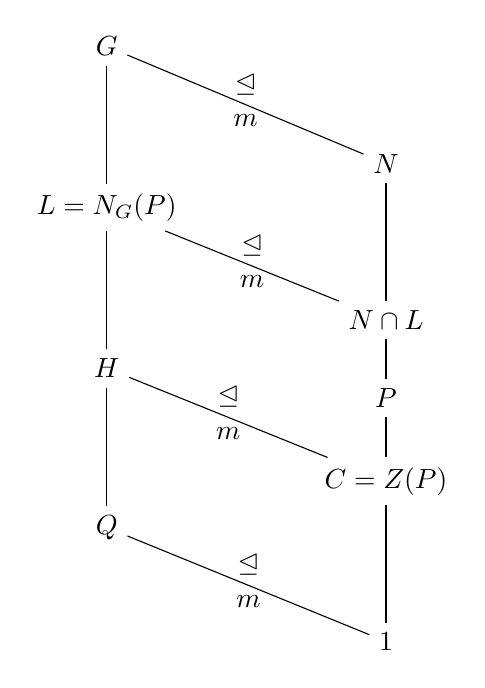
\begin{tikzpicture}[node distance=2cm, scale=1, transform shape]
				\title{Diagrama}
				
				\node(G) {$G$};
				\node(N)		[below right = 1cm and 3cm of G] {$N$};
				\node(L)		[below = 1.5cm of G] {$L=N_{G}(P)$};
				\node(NcL)	[below = 1.5cm of N] {$N\cap L$};
				\node(P)		[below = 0.5cm of NcL] {$P$};
				\node(C)		[below = 1.5cm of NcL] {$C=Z(P)$};
				\node(H)		[below = 1.5cm of L] {$H$};
				\node(Q)		[below = 1.5cm of H] {$Q$};
				\node(C1)	[below = 1.5cm of C] {$1$};
				
				
				\draw(G)-- node[above]{$\norm$} node[below]{$m$}(N);
				\draw(G)--(L);
				\draw(N)--(NcL);
				\draw(L)-- node[above]{$\norm$} node[below]{$m$}(NcL);
				\draw(L)--(H);
				%\draw(NcL)--(C);
				\draw(NcL)--(P);
				\draw(P)--(C);
				\draw(H)-- node[above]{$\norm$} node[below]{$m$}(C);
				\draw(H)--(Q);
				\draw(Q)-- node[above]{$\norm$} node[below]{$m$}(C1);
				\draw(C)--(C1);
	
			\end{tikzpicture}
		\end{figure}
		
		\textit{(ii) Conjugación (Caso N resoluble)}. Sean $Q_1$ y $Q_2$ subgrupos de $G$ de orden $m$. Como $N$ es resoluble $N'\neq N$, $N'\car N\norm G$ y por tanto, $N'\norm G$. Aplicando el caso abeliano a $N/N'$ y $G/N'$, $Q_1N'/N'$ y $Q_2N'/N'$ son conjugados. Por tanto, existe $g_1\in G$ tal que $Q_1^{g_1} \leq Q_2 N'$. % aclarar esto
		$Q_1^{g_1}$ y $Q_2$ son subgrupos de orden $m$ en $Q_2N'$ y aplicando inducción sobre la longitud derivada de $N$ se llega a $Q_1^{g_d}\leq Q_2N^{(d)} = Q_2$.
		
		\textit{(iii) Conjugación (Caso G/N resoluble)}.
	\end{demostracion}
\end{teorema}

%\apendices



%\incluir{Bibliografia}

\end{document}